%%
%% This is file `example/ch_intro.tex',
%% generated with the docstrip utility.
%%
%% The original source files were:
%%
%% install/buptgraduatethesis.dtx  (with options: `ch-intro')
%% 
%% This file is a part of the example of BUPTGraduateThesis.
%% 

\chapter{基于递归注意力机制的模型}
本章主要提出了一种基于递归注意力机制的模型。首先章节~\ref{sec:ran_intro}描述了算法的研究背景;接着,在章节~\ref{sec:ran_algori}中介绍了基于递归注意力机制的模型结构,包括算法的设计、模型的学习与预测等过程;章节~\ref{sec:ran_exper}中介绍实验设置相关内容,对实验数据集,对比方法等进行介绍;章节~\ref{sec:ran_exper_result}对实验结果进行分析,章节\ref{sec:ran_analysis}对实验结果进行进一步的分析和讨论,章节\ref{sec:ran_conclu}对本章内容进行总结。

\section{引言}
\label{sec:ran_intro}
法条语义信息(例如,法条的定义)为法官进行正确的决策提供了有效的属性信息。表~\ref{t:similar_article}展示了两个相似的法条。具体来讲,给定案情描述,对法官来说,一个正常的步骤是法官首先浏览案情,之后浏览所有的法条,挑选与给定案情相关的候选法条(例如,刑法第263条和刑法第264条都与盗窃罪相关,它们在法条定义中有相似的文本描述)。之后通过对案情和候选法条进行详细的语义分析最终挑选正确的法条。这个过程往往会重复若干次之后才能得到最终的判决结果。

\begin{table}[htb]
    \caption{相关法条变}
    \label{t:similar_article}
    \centering
    \begin{tabular}{lp{12cm}p{7cm}}
    \hline
    &\emph{\textbf{刑法第一百九十七条}: 使用伪造、变造的国库券或者国家发行的其他有价证券,进行\emph{\textbf{诈骗}}活动,数额较大的,处五年以下有期徒刑或者拘役... \newline
    \textbf{刑法第一百九十一条}: 明知是毒品犯罪、黑社会性质的组织犯罪、恐怖活动犯罪、走私犯罪、贪污贿赂犯罪、破坏金融管理秩序犯罪、\emph{\textbf{金融诈骗}}犯罪的所得及其产生的收益,为掩饰、隐瞒其来源和性质,有下列行为之一的,没收实施以上犯罪的所得及其产生的收益...}\\
    \hline
    \end{tabular}
\end{table}

之前的工作,通常忽略了标签语义信息进行预测。此外,案情与法条语义之间的重复迭代信息被忽略,因此之前的算法性能是十分有限的。在本章中,为了解决这些问题,本课题提出了一种递归注意力网络(简称RNN)。具体来讲,RAN利用LSTM将案情描述和法条定义映射到一个低维空间。自注意力机制用来获取案情和法条自身的内部信息。协同注意力机制用来选择有效的语义信息对案情和法条进行正确的匹配。最后一个递归单元用来建模案情和法条之间的交互信息。

总体来说,本章主要贡献如下:
\begin{itemize}
    \item 本章将判决预测问题转换为匹配问题,以便分析法条定义与案情描述之间的语义信息。
    \item 本章设计了一种新型递归单元用于建模法条定义与案情描述之间的重复语义交互信息。
    \item 本章在真实数据上进行了有效的实验验证,本章模型结果有效超过了基线模型,进一步的分析证明了本章提出的递归注意力机制方法的有效性。
\end{itemize}

\section{RAN算法设计}
\label{sec:ran_algori}

在本节中,针对提出了RAN模型进行详细的介绍,其模型结果如图~\ref{fig:ran_model},之后对算法的学习和预测过程进行介绍。
\begin{figure*}[htbp]
    \centering
    \includegraphics[scale=0.45,viewport=0 30 980 500,clip=true]{./sources/RAN.eps}
    \vspace{-10pt}
    \caption{\label{fig:ran_model} 递归注意力网络(RAN)模型结构图 }
    \vspace{-5pt}
\end{figure*}

RAN模型主要包含四层,编码层利用\textbf{LSTM}将案情描述和法条定义映射到低维语义空,自注意力机制产出两者的加权特征表达,递归层建模法官交替阅读案情描述和法条的过程,以便获得重复的交替语义特征,最后输出层产出模型的预测结果。

\subsection{编码层}
让 $x^{(i)} = {\{w_1, w_2, w_3, \dots, w_m\}}$表示有$m$个词的案情描述, $l^{(j)} = {\{w_1, w_2, w_3, \dots, w_n\}}$表示有$n$个词的法条定义,$w_i$代表第$i$个词的词袋表示,让$\textbf{V}^I=\{\vec{v}^I_t\in \mathbb{R}^{D_v}|t=1,\dots,N\}$表示所有词向量的连续空间。

针对每个案情描述和法条定义,本课题将词向量聚合作为案情表示和标签表示,一个双向LSTM(简称Bi-LSTM)用来计算每个词在时刻$t$的隐层状态,其计算过程如公式~\ref{eq:lstm}:
\begin{equation}\label{eq:lstm}
    \begin{aligned}
        \overrightarrow{h_t}&=\overrightarrow{\text{LSTM}}(\overrightarrow{h}_{t-1}, w_t)\\
        \overleftarrow{h_t}&=\overrightarrow{\text{LSTM}}(\overleftarrow{h}_{t-1}, w_t)\\
    \end{aligned}
\end{equation}

利用Bi-LSTM,本模型通过拼接两个方向的LSTM的隐层状态组成第$i$个词的隐层表示,$\vec{v}_t=[\overrightarrow{h_t};\overleftarrow{h_t}]$,之后案情序列 $x^{(i)}$ 和法条序列$l^{(j)}$被分别映射到连续的空间$\textbf{H}_e^{(i)}=[\vec{v}_e^{i}(1), \vec{v}_e^{i}(2), \dots, \vec{v}_e^{i}(m)]$,
$\textbf{H}_a^{(i)}=[\vec{v}_a^{i}(1), \vec{v}_a^{i}(2), \dots, \vec{v}_a^{i}(n)]$。
\subsection{自注意力层}

在案情描述文档中,不同的词拥有不同的重要程度用于支持法官判决,法官需要详细的阅读案情描述来确认其中的重要犯罪情节。相似的,法条定义中不同的词也有不同的重要程度。在刑法中,有许多易混淆的罪名,比如盗窃罪和抢劫罪,故意杀人和过世致人死亡,它们在法条定义中只有一些细微的差别。例如,是否在非法占有过程中使用暴力,犯罪者在非法占有中使用暴力,是否是由犯罪者故意造成受害人死亡。在进行判决的过程中,法官需要根据法条定义中的差异信息来确认被告人违反了哪些法条。

受自注意力机制\cite{VaswaniSPUJGKP17}的启发,给定案情描述或者法条定义,本课题根据词的重要程度针对文本中的不同词分配不同的权重。这种机制将查询和一系列键值对映射到输出,查询,键,值和输出拥有同样的维度。这本模型中,查询,键,值都是编码层的输出$\textbf{H}_e^{(i)}$ and $\textbf{H}_a^{(j)}$,多头注意力机制允许模型对来自不同子空间的信息在不同位置进行加权。权重计算过程如下:
\begin{equation}\label{eq:self_attention}
    head_i = Attention(Q,K,V) = softmax(\frac{QK^{T}}{\sqrt{d_k}})V
\end{equation}

\begin{equation}\label{eq:multi_head_attention}
    \begin{aligned}
        &MultiHead(Q,K,V) = \\
        &Concat(head_1,\dots,head_h)W^{O} \\            
    \end{aligned}
\end{equation}

其中,$Q,K,V$代表打包的查询,键值,$d_k$和$d_v$代表查询和值的维度,投影$W_i^Q \in \mathbb{R}^{d_{model} \times d_k}, W_i^K 
\in \mathbb{R}^{d_{model} \times d_k},W_i^V \in \mathbb{R}^{d_{model} \times d_v}, W^O \in \mathbb{R}^{hd_v \times d_{model}}$是参数矩阵。利用自注意力机制,本课题将$\textbf{H}_e^i$和$\textbf{H}_a^j$映射到另外一个相当大小的序列空间 $\textbf{H}_{e,s}^{(i)} = [\vec{v}_{e,s}^{(i)}(1), \vec{v}_{e,s}^{(i)}(2), \dots, \vec{v}_{a,s}^{(t)}(t)]$. 和 $\textbf{H}_{a,s}^{(j)}=[\vec{v}_{a,s}^{(j)}(1), \vec{v}_{a,s}^{(j)}(2), \dots, \vec{v}_{a,s}^{(j)}(t)]$。
\subsection{递归层}
在司法领域,法官需要仔细阅读案情描述以便获得重要信息,以便找出相关法条作为候选,之后针对案情描述和相关法条进行详细的分析,得到最终的判决结果,这个过程通过需要重复多次来进行最后的决策。与Cui等人\cite{CuiCWWLH17}提出的不同,不是利用简单的源文本到目标文本之间的交互信息,本课题设计了一种递归注意力机制单元用于建模法官的重复阅读行为。

通过自注意力机制,本课题获得了案情和标签的词级别的表达,分别是$\textbf{H}_{e,s}^{(i)}$ 和 $\textbf{H}_{a,s}^{(j)}$。本课题通过聚合操作获取标签句子级别的表达,其计算过程如下:
\begin{equation}\label{eq:label vector}
    \begin{aligned}
        & \vec{v}_{a,m}(j)=\frac{1}{m}\sum\limits_{t}\vec{v}_{a,m}^{(j)}(t) \\
        & \textbf{H}_{a,m} = [\vec{v}_{a,m}(1), \vec{v}_{a,m}(2), \dots, \vec{v}_{a,m}(|C|)] \\
    \end{aligned}
\end{equation}

其中,$\textbf{H}_{a,m}$代表标签全局表达,由每个标签的表达聚合而来。

本课题以$\vec{v}_{a,m}(j)$作为$\textbf{H}_{a,m}$的第$j$个元素,以$\vec{v}_{e,s}^{(i)}(k)$作为$\textbf{H}_{e,s}^{(i)}$的第$k$个元素,之后本课题对标签表达和案情词级别的表达构造匹配得分矩阵$\textbf{M}^{(i)}$,计算方法如下:
\begin{equation}\label{eq:match score}
    \textbf{M}^{(i)}(j,k) = \vec{v}_{a,m}(j) \cdot \vec{v}_{e,s}^{(i)}(k)
\end{equation}

其中,$M^{(i)} \in \mathbb{R}^{|\textbf{H}_{a,m}|*|\textbf{H}_{e,s}^{(i)}|}$,每个元素代表交互得分。

获得匹配得分矩阵$\textbf{M}^{(i)}$之后,采用列softmax函数获得每列的概率分布。其中每列代表独立的注意力值,之后采用$\alpha(t) \in \mathbb{R}^{|C|}$代表每个案情中的词在$t$时刻标签级别的注意力,它可以看作是案情词到标签的权重分布,其计算过程如下:
\begin{equation}\label{eq:alpha attention}
    \begin{aligned}
        & \alpha(t)=softmax(\textbf{M}^{(i)}(1,t), \textbf{M}^{(i)}(2,t), \dots, \textbf{M}^{(i)}(|\textbf{H}_{a,m}|,t)\\
        & \alpha=[\alpha(1),\alpha(2),\dots,\alpha(|\textbf{H}_{e,s}^{(i)}|)] \\
    \end{aligned}
\end{equation}

之后对所有的$\alpha(t)$进行平均得到平均标签级别的注意力$\alpha^{'} \in \mathbb{R}^{|H_{a,m}|}$,其中平均操作不会破坏正则化分布:
\begin{equation}\label{eq:avg alpha}
    \alpha{'}=\frac{1}{|\textbf{H}_{a,m}|}\sum\limits_{i=1}^{|\textbf{H}_{a,m}|}\alpha(t) \\
\end{equation}

通过同样的方式,本课题可以使用行softmax获取标签到案情中每个词的注意力值$\beta^{'} \in \mathbb{R}^{|\textbf{H}_{e,s}^{(i)}|}$,其计算过程如下:
\begin{equation}
    \begin{aligned}
        & \beta(t)=softmax(\textbf{M}(t,1), \textbf{M}(t,2), \dots, \textbf{M}(t, |\textbf{H}_{e,s}^{(i)}|)\\
        & \beta = [\beta(1), \beta(2), \dots, \beta(|\textbf{H}_{a,m}|)] \\
    \end{aligned}
\end{equation}
\begin{equation}
    \beta{'}=\frac{1}{|\textbf{H}_{e,s}^{(i)}|}\sum\limits_{i=1}^{|\textbf{H}_{e,s}^{(i)}|}\beta(t)
\end{equation}

目前为止,本课题已经获得了双向的注意力矩阵$\alpha^{'}$ 和 $\beta^{'}$。本课题的研究动机是模拟法官交替阅读案情和法条定义的过程。因此提出了一种递归的结构。直观上来讲,这个操作通过不断进行循环可以学习到重要的交互语义信息。其计算过程如下:

\begin{equation}\label{eq:recurrent}
    \begin{aligned}
        % & \textbf{S} = \textbf{S} + \textbf{S}\textbf{W}\beta^{'} \\
        % & \textbf{C} = \textbf{C} + \textbf{C}\textbf{W}\alpha^{'} \\
        & \textbf{H}_{e,r}^{(i)} = r(\textbf{H}_{e,s}^{i} + \textbf{H}_{e,s}^{i}\textbf{W}^{\alpha{'}}\alpha{'}) \\
        & \textbf{H}_{a,r} = r(\textbf{H}_{a,m} + \textbf{H}_{a,m}\textbf{W}^{\beta{'}}\beta{'}) \\
    \end{aligned}
\end{equation}

其中 $\textbf{W}^{\alpha{'}}$ 和 $\textbf{W}^{\beta{'}}$是维度变换矩阵, $r$代表递归操作。如公式~\ref{eq:recurrent}中的描述,本模型重复这个过程若干次,最终通过案情和标签描述之间语义的重复交互获得最终正确的匹配。


\subsection{输出层}
为了整合案情和相关法条定义两部分信息,在输出层中,对于给定实例,本课题同时采用案情和标签两部分特征进行最终结果预测。在所有标签上进行得分预测的过程如下:
\begin{equation}
    \begin{aligned}
        % &  \textbf{s} = avg(\textbf{S}) \\
        % & \textbf{c} = avg(\textbf{C}) \\
        % &  \textbf{v} = \textbf{c} \oplus \textbf{s}\\
        % & f = sigmoid(\textbf{W}^{v}\textbf{v} + \textbf{b}^{v}) \\
        & \vec{v}_{e,r}^{(i)} = g(H_{e,r}^{(i)}) = \frac{1}{m}\sum\limits_{t}\vec{v}_{e,r}^{(i)}(t) \\
        & \vec{v}_{a,r} = g(H_{a,r}) = \frac{1}{m}\sum\limits_{t}\vec{v}_{a,r}(t) \\
        & \vec{v}_{f}^{(i)} = \vec{v}_{e,r}^{(i)} \oplus \vec{v}_{a,r} \\
        & \vec{v}_{o}^{(i)} = \textbf{W}^{o}\vec{v}_{f}^{(i)} + b^{o}
    \end{aligned}
\end{equation}

其中,$g$代表平均操作,$\vec{v}_{e,r}^{(i)}$代表案情文本特征表达,$\vec{v}_{a,r}$代表所有法条的平均特征表达,它代表法条标签的全局特征。$\oplus$代表拼接操作,$\textbf{W}^{o}$ 和 $\textbf{b}^{o}$是可学习的参数。

\subsection{模型学习与预测}
为了学习\textbf{RAN}的模型参数,采用随机梯度下降进行参数更新,在训练过程中采用二元交叉熵作为损失,其计算结果如下:
\begin{equation}\label{eq:loss}
    \begin{aligned}
        & l = -\frac{1}{n}\sum\limits_{i=1}^{n}\sum\limits_{j=1}^{|\mathcal{C}|}[Y^{(i)}(j)log(\sigma(\vec{v}^{(i)}_{o}(j))) \\
        & + (1 - Y^{(i)}(j))log(1 - \sigma(\vec{v}^{(i)}_{o}(j)))] \\
    \end{aligned}
\end{equation}

其中$\sigma$是sigmoid函数$\sigma(x)=\frac{1}{1 + e^{-x}}$,$Y^{(i)}(j) \in \{0, 1\}$是针对实例$x^{(i)}$的第$j$个标签的真实值。

使用学习到的参数,分类策略如算法~\ref{alg:ran_algo}所示:
\begin{algorithm}[htb]
    \caption{RAN模型学习框架}
    \label{alg:ran_algo}
    \begin{algorithmic}[1]
    % \Require
    % The set of positive samples for current batch, $P_n$;
    % The set of unlabeled samples for current batch, $U_n$;
    % Ensemble of classifiers on former batches, $E_{n-1}$;
    % \Ensure
    % Ensemble of classifiers on the current batch, $E_n$;
    \State 随机初始化模型参数 $\Theta=\{\textbf{W}^{D_V\times |C|},\textbf{V}$\}
    \label{code:fram:initialize parameters}
    \State iter = 0
    \label{code:fram:begin}
    \Repeat
    \label{code:fram:repeat}
        \State $iter \leftarrow iter+1$
        \label{code:fram:re_value}
        \For{$i = 1,...,|X|$}
        \label{code:fram:for1}
            \State 针对实例 $x^{(i)}$
            \label{code:fram:task_join1}
            \State 编码案情描述和法条定义 $H_e^{(i)}$, $H_a$
            \label{code:fram:encode}
            % \State self attention encode
            % \label{code:fram:self_at_encode}
            \State set $n_{layer} = 3$
            \label{code:fram:recurrent_layer}
            \Repeat
            \label{code:fram:repeat_recurrent}
                \State $n_{layer} \leftarrow n_{layer} - 1$ 
                \label{code:fram:iter_layer}
                \State 计算交互信息
                \label{code:fram:compute_iteraction}
            \Until{$n_{layer} < 0$}
            \State  通过公式(\ref{eq:loss})计算模型梯度$\nabla(\theta)$
            \label{code:fram:com_grad}
            \State 通过$\theta \leftarrow \theta + \epsilon \nabla(\theta)$更新模型参数
            \label{code:fram:update_grad}
        \EndFor
        
    \Until{(收敛或者$t > num$)}
    \State
    \Return $\{\textbf{W}^{D_V\times |C|},\textbf{V}^I\}$;
    \end{algorithmic}
\end{algorithm}

针对每个实例$x^{(i)}$,可以获得每个标签$Y^{(i)}(j)$的概率分布。结合阈值$t$,可以得到$x^{(i)}$的预测标签集合,其计算过程如下:
\begin{displaymath}
    Y^{(i)}(j)=\left\{
    \begin{aligned}
    1 &, \quad \textbf{if} \quad \mathbb{I}(\sigma(v_{o}^{(i)}(j))) > t \\
    0 &, \quad \textbf{else} \\
    \end{aligned}
    \right.
\end{displaymath}

其中,$\mathbb{I}$是索引函数,概率大于$t$的标签作为与实例$x^{(i)}$相关的标签。

\section{实验设置}
\label{sec:ran_exper}
\subsection{数据集介绍}
本模型在三个数据集上进行了实验验证:
\begin{itemize}
    \item \textbf{CJO}:这个数据集包含114576个样本,是本课题从中国裁判文书网\footnote{https://wenshu.court.gov.cn/}进行收集的数据,并且每个样本已经被结构化为案情,判决结果等及部分。
    \item \textbf{CAIL samll}:这个数据集是为司法判决竞赛开发的数据集,它由最高人民法院公布~\footnote{http://cail.cipsc.org.cn/},包含2043231个样本。这个数据集包含事实描述,以及对应的相关法条,判决结果,罚金等。
    \item \textbf{CAIL2018}:这个数据集是一个公开的大型数据集\cite{zhong2018legal}用于司法判决预测,CAIL2018包含超过200万个样本,是现有的同类数据集的若干倍大。
\end{itemize}

三个数据集的统计分析如表~\ref{t:ran_statistic}所示。最后本课题将所有数据以$8:2$划分为不重叠的两部分,训练集和测试机。
\begin{table}[htb]
\centering
\caption{三个数据集统计表}
\label{t:ran_statistic}
\begin{tabular}{lllll}
\hline
\multirow{2}{*}{数据集} & \multirow{2}{*}{\begin{tabular}[c]{@{}l@{}}样本\\ 个数\end{tabular}} & \multirow{2}{*}{\begin{tabular}[c]{@{}l@{}}法条\\ 个数\end{tabular}} & \multirow{2}{*}{\begin{tabular}[c]{@{}l@{}}平均案情\\ 描述长度\end{tabular}} & \multirow{2}{*}{\begin{tabular}[c]{@{}l@{}}平均\\ 标签个数\end{tabular}} \\
                     &                                                                  &                                                                  &                                                                      &                                                                    \\ \hline
CJO                  & 114,576                                                          & 137                                                              & 825                                                                  & 1.17                                                               \\
CAIL small           & 204,231                                                          & 183                                                              & 263                                                                  & 1.27                                                               \\
CAIL2018             & 1,710,856                                                        & 183                                                              & 279                                                                  & 1.04                                                               \\ \hline
\end{tabular}
\end{table}


\subsection{模型评估}
本课题采用以下模型进行实验对比:
\begin{itemize}
    \item \textbf{ML-KNN},\textbf{BR},\textbf{CC}均在章节~\ref{sec:dpam_exper}中进行过详细介绍,此处不再赘述。
    \item \textbf{CNN}:一种二阶多标签分类模型,使用卷积神经网络作为输入特征\cite{Kim14},之后输入到带有sigmoid的全连接模型中在所有标签下得到概率分布。采用多标签软边界损失进行优化。
    \item \textbf{BiLSTM}:BiLSTM\cite{graves2005framewise}同样是一种二阶方法,该方法是一种常用的用于建模长期依赖的方法,本课题采用于\textbf{CNN}类似的方法进行继承。
    \item \textbf{DPAM}:DPAM\cite{DPAM}本文在~\ref{chapter:3}提出的另一种基于神经网络的模型,采用注意力机制获取标签之间的关联关系。
\end{itemize}

针对所有模型,本课题设置句子最大长度为$500$个词。对于浅层模型来说,这些模型采用词袋和TF-IDF特征当作输入,使用卡方检验选取前$5000$个特征\cite{luo2017learning}。对于其他模型,本课题将案情表达和法条表达设置为$256$维特征。本课题采用一个$100000$大小的词典,词典外的词采用一个特殊的词$unk$进行替换。使用Adam作为优化器进行损失优化,设置学习率为$0.001$,两个动量参数分别设置为$0.9$和$0.999$。具体地, 

\section{实验结果}
\label{sec:ran_exper_result}
\subsection{与基线模型的实验对比}
本课题将提出的\textbf{SAN}模型与baseline进行了对比,在三个数据集上的性能结果如表~\ref{t:ran_main}所示:\begin{table*}[htbp]
    \centering
    \caption{RAN与基线模型实验比较表}
    \label{t:ran_main}
    \setlength{\tabcolsep}{0.65mm}
    \begin{tabular}{@{}c|c|cccc|cc|c|c|c@{}}
        \toprule
        \multirow{3}{*}{\textbf{数据集}} & \multirow{3}{*}{\textbf{指标}} & \multicolumn{4}{c|}{\multirow{2}{*}{\textbf{\begin{tabular}[c]{@{}c@{}}浅层 \\ 模型\end{tabular}}}} & \multicolumn{2}{c|}{\multirow{2}{*}{\textbf{\begin{tabular}[c]{@{}c@{}}神经网络 \\ 模型\end{tabular}}}} & \multirow{2}{*}{\textbf{\begin{tabular}[c]{@{}c@{}}注意力 \\ 模型\end{tabular}}} & \multirow{2}{*}{\textbf{\begin{tabular}[c]{@{}c@{}}本\\ 模型\end{tabular}}} & \multirow{3}{*}{\textbf{提升}} \\
                                          &                                   & \multicolumn{4}{c|}{}                                                                                   & \multicolumn{2}{c|}{}                                                                                                &                                                                                            &                                                                               &                                   \\
                                          &                                   & MLKNN                    & BR                       & CC                      & SVM                     & TextCNN                                                   & BiLSTM                                                   & DPAM                                                                                       & RAN                                                                          &                                   \\ \midrule
                                          & MP                                & 59.49                    & 74.28                    & 72.33                   & 67.68                   & 78.53                                                     & 78.81                                                    & 79.39                                                                                      & \underline{\textbf{81.34}}                                                                & \textbf{1.95}                     \\
                                          & MR                                & 32.14                    & 50.84                    & 53.22                   & 51.37                   & 54.16                                                     & 54.96                                                    & 55.60                                                                                      & \underline{\textbf{55.59}}                                                                & \textbf{0.09}                     \\
        \textbf{CJO}                      & MF                               & 38.85                    & 57.41                    & 58.60                   & 55.77                   & 61.40                                                     & 62.17                                                    & 62.79                                                                                      & \underline{\textbf{63.28}}                                                               & \textbf{0.49}                     \\
                                          & JS                                & 53.25                    & 79.40                    & 82.02                   & 83.55                   & 80.25                                                     & 80.40                                                    & 80.76                                                                                      & \textbf{80.81}                                                                & \textbf{0.05}                     \\
                                          & MP                                & 31.75                    & 41.59                    & 42.12                   & 43.07                   & 78.32                                                     & 79.93                                                    & 80.35                                                                                      & \underline{\textbf{81.23}}                                                                & \textbf{0.88}                     \\
                                          & MR                                & 20.11                    & 30.23                    & 32.49                   & 39.66                   & 54.73                                                     & 57.77                                                    & 62.03                                                                                      & \underline{\textbf{64.90}}                                                                & \textbf{2.87}                     \\
        \textbf{CAIL small}               & MF                               & 22.93                    & 33.57                    & 35.58                   & 40.14                   & 61.35                                                     & 63.98                                                    & 67.42                                                                                      & \underline{\textbf{69.49}}                                                                & \textbf{2.07}                     \\
                                          & JS                                & 38.85                    & 59.74                    & 62.59                   & 71.98                   & 74.12                                                     & 75.09                                                    & 76.00                                                                                      & \underline{\textbf{77.42}}                                                                & \textbf{1.42}                     \\
                                          & MP                                & 28.88                    & 40.42                    & 38.91                   & 40.82                   & 74.86                                                     & 75.05                                                    & 75.26                                                                                     & \underline{\textbf{77.69}}                                                                & \textbf{2.43}                     \\
                                          & MR                                & 16.59                    & 26.95                    & 28.86                   & 31.53                   & 57.43                                                     & 57.79                                                    & 58.04                                                                                      & \underline{\textbf{58.69}}                                                                & \textbf{0.65}                     \\
        \textbf{CAIL2018}                 & MF                               & 19.68                    & 30.65                    & 31.59                   & 34.01                   & 62.91                                                     & 63.01                                                    & 63.33                                                                                      & \underline{\textbf{64.88}}                                                               & \textbf{1.55}                     \\
                                          & JS                                & 70.28                    & 88.34                    & 90.57                   & 90.92                   & 94.61                                                     & 94.61                                                    & 94.39                                                                                      & \underline{\textbf{94.68}}                                                                & \textbf{0.29}                     \\ \bottomrule
        \end{tabular}
\end{table*}

其中MP,MR,MF和JS分别代表Macro-P,Macro-R,Macro-F1和杰卡德相关系数(所有数值的百分比符号均被省略)。每行最好的实验结果用下划线进行了标注,最后一列代表与最好的基线模型相关性能提升的多少。本课题将对比的模型分为三个大类别,浅层模型,基于神经网络的模型以及基于注意力机制的模型。从结果中,可以得到以下结论:
\begin{itemize}
    \item 毫不惊讶,\textbf{MLKNN}和\textbf{BR}的在所有指标上结果最差,因为这两种方法将多标签分类转换为单标签分类。
    \item \textbf{CC}方法比\textbf{MLKNN}和\textbf{BR}要稍好,这是由于\textbf{CC}建模了标签关联。
    \item 基于神经网络的方法性能明显好于大多数浅层模型。以\textbf{TextCNN}为例,与最好的浅层模型(CC)相比,在CAIL small上MP,MR,MF, JS分别提升了$36.2\%$,$22.24\%$,$25.77\%$和$11.53\%$。它证明神经网络模型可以有效建模语义信息。
    \item 基于注意力机制的模型\textbf{DPAM}的结果好于大多数模型(除过\textbf{RAN}),这表明引入法条语义信息是一种很好的整合案情和法条信息的方式。
    \item \textbf{RAN}在所有指标上获得了最好的性能。在CAIL Small上与\textbf{DPAM}相比,MP,MR,MF,JS的结果提升分别是$0.88\%$, $2.5\%$, $2.07\%$, $1.42\%$。
\end{itemize}

这个结果能有效支撑本模型的假设,建模案情和法条之间重复的交互语义信息是非常重要和有效的。

\section{分析与讨论}
\label{sec:ran_analysis}
本课题在模型上进行了进一步的分析。在本节中,本课题首先挖掘了递归层数对结果的影响,之后利用消融实验探索了不同模型层的有效性。
\begin{figure*}[hbtp]
    \centering
    % \includegraphics[scale=0.5,viewport=0 30 980 500,clip=true]{./sources/n_layers.eps}
    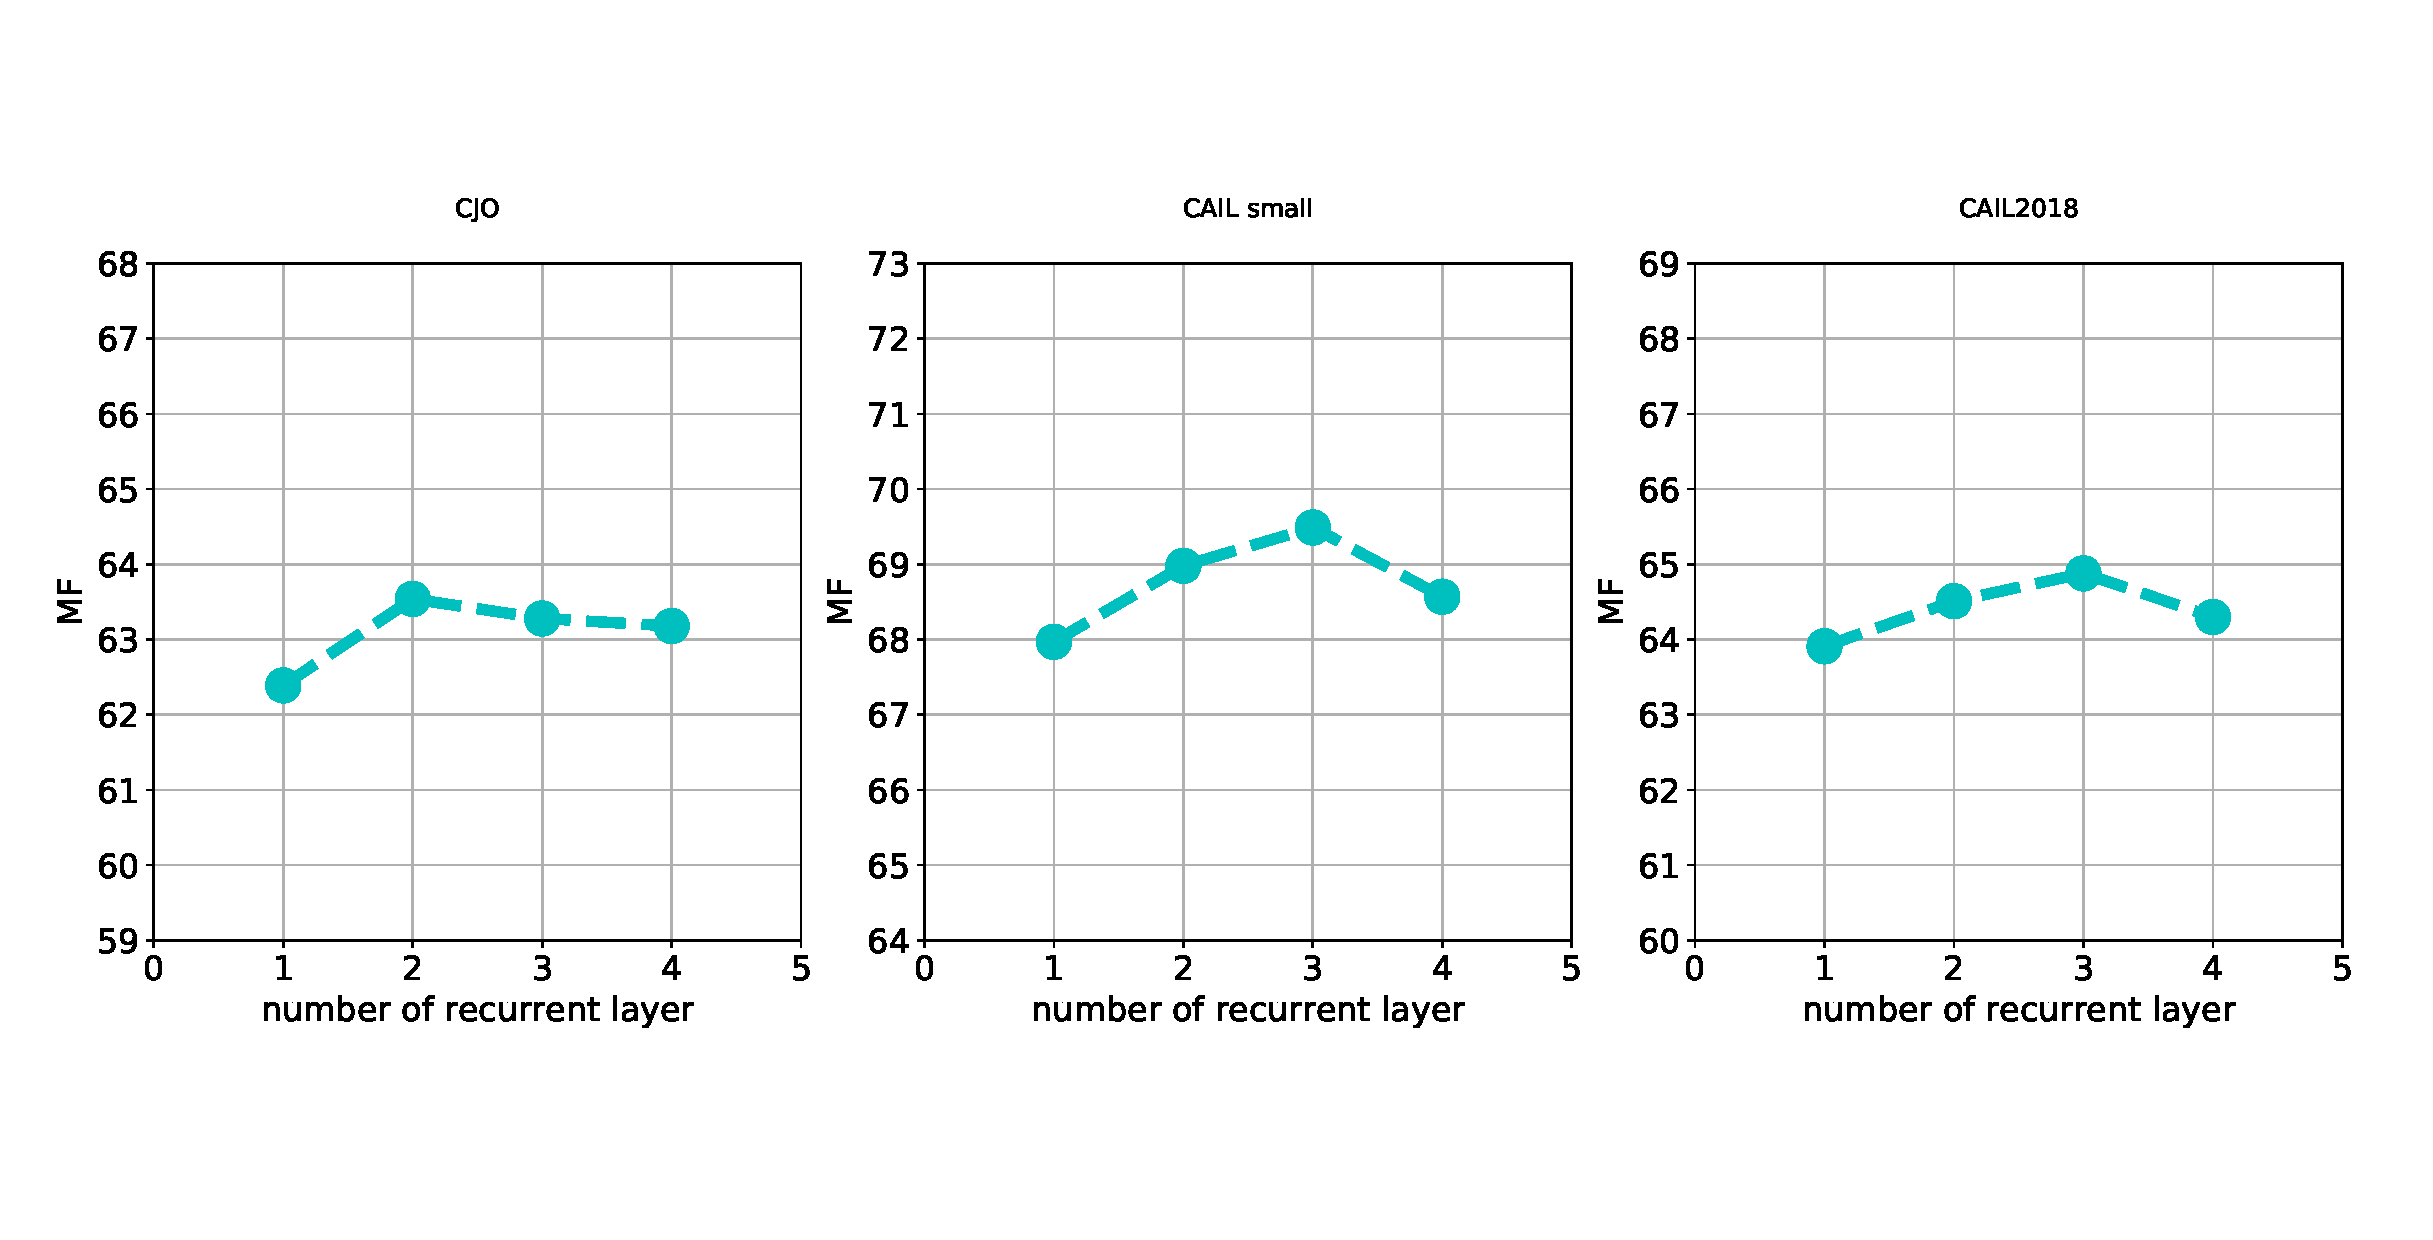
\includegraphics[scale=0.39, clip=true]{./sources/3_recurrent_layers2.eps}
    \vspace{-10pt}
    \caption{\label{fig:n_layers} 递归层数影响实验图}
    \vspace{-5pt}
\end{figure*}

\subsection{递归层影响分析}
本课题在递归交互层数$n \in \{1,2,3,4\}$的情况下在三个数据集上进行实验,实验结果如图~\ref{fig:n_layers}所示,从结果可以得到以下结论:
\begin{itemize}
    \item 随着递归层数的增多,结果有所提升。
    \item 当层数增加到一定程度,性能提升变得非常有限,并且需要更多的计算资源。
    \item 当递归层数增加到3层以上,结果开始下降。
\end{itemize}



\subsection{消融实验}
为了进一步验证,本课题进行了不同程度的消融实验,将递归层移去(简称\textbf{R-r}),将自注意力层移去(简称R-s)分别进行实验。实验结果如表~\ref{t:ablation}所示:
\begin{table}[htbp]
    \centering
    \caption{CAIL small数据集消融实验}
    \label{t:ablation}
    \begin{tabular}{ccccccc}
        \hline
        \textbf{数据集}                                                                & \textbf{方法} & \textbf{MP} & \textbf{MR}    & \textbf{MF}    & \textbf{JS} \\ \hline
        \multirow{4}{*}{\textbf{CJO}}                                                   & \textbf{DPAM}   & 79.39       & 55.60 & 62.79  & 80.76       \\
                                                                                        & \textbf{R-s}    & 80.36       & 55.02 & 62.85  & 80.77       \\
                                                                                        & \textbf{R-r}    & 78.78       & 54.56 & 61.97  & 80.35       \\
                                                                                        & \textbf{RAN}    & 81.34       & 55.59 & 63.28  & 80.81       \\
        \multirow{4}{*}{\textbf{\begin{tabular}[c]{@{}c@{}}CAIL small\end{tabular}}} & \textbf{DPAM}   & 80.35       & 62.03 & 67.42  & 76.00       \\
                                                                                        & \textbf{R-s}    & 80.2        & 64.94 & 68.98  & 76.58       \\
                                                                                        & \textbf{R-r}    & 79.37       & 62.08 & 66.75  & 76.93       \\
                                                                                        & \textbf{RAN}    & 81.23       & 64.9  & 69.49  & 77.42       \\
        \multirow{4}{*}{\textbf{\begin{tabular}[c]{@{}c@{}}CAIL2018 \end{tabular}}}   & \textbf{DPAM}   & 75.26       & 58.04 & 63.33  & 94.39       \\
                                                                                        & \textbf{R-s}    & 75.3        & 58.06 & 63.9   & 94.64       \\
                                                                                        & \textbf{R-r}    & 74.33       & 57.54 & 62.65  & 94.41       \\
                                                                                        & \textbf{RAN}    & 77.69       & 58.69 & 64.88  & 94.68       \\ \hline
        \end{tabular}
\end{table}

本课题得到以下结论:\
\begin{itemize}
    \item 仅仅保持自注意力层,实验结果比\textbf{DPAM}要差。这是由于缺乏标签相关信息无法有效区分易混淆的法条标签。
    \item 仅仅保存递归层,实验结果稍好于\textbf{DPAM}。这是由于递归层可以有效利用案情和法条标签之间的交互信息。
    \item 结合自注意力层和递归层,\textbf{RAN}通过自注意力层获得案情和法条独立的重要信息,之后通过递归层获得交互信息,可以获得更有效的信息帮助提高模型性能。
\end{itemize}
这进一步证明了递归层可以有效建模获取重复的语义信息用于提升判决预测的性能。
\section{本章小结}
\label{sec:ran_conclu}
在本章节张,本课题提出了一种递归注意力网络,可以模拟法官重复交替阅读法案和法条的过程,这种方法可以有效利用案情描述和法条定义之间的交互语义特征,扩展实验证明提出的模型性能远好于其他模型。进一步的分析证明本模型不仅能够获取标签关联信息,还能通过递归单元获取多层次的注意力信息。

% \chapterbib
